\documentclass[11pt]{beamer}
\usetheme{Singapore}
%\usecolortheme{dove}
\usepackage{etoolbox}
\usepackage{ragged2e}
\usepackage[utf8]{inputenc}
\usepackage[italian]{babel}
\usepackage{scrextend}
\usepackage{tikz}
\usepackage{adjustbox}
\AtBeginSection[]{\subsection{}}
\usetikzlibrary{shapes.geometric, arrows}
\tikzstyle{startstop} = [rectangle, 
rounded corners, 
minimum width=1cm, 
minimum height=.5cm,
text centered, 
draw=black, 
fill=red!30]

\tikzstyle{io} = [trapezium, 
trapezium left angle=70, 
trapezium right angle=110, 
minimum width=1cm, 
minimum height=0.5cm, 
text centered, 
draw=black, 
fill=blue!30
]
\tikzstyle{process} = [rectangle, 
minimum width=1cm, 
minimum height=.5cm, 
text centered, 
draw=black, 
fill=orange!30, 
text width=0.95\linewidth]

\tikzstyle{process_red} = [rectangle, 
minimum width=3cm, 
minimum height=1cm, 
text centered, 
draw=black, 
fill=red!70, 
text width=0.95\linewidth]

\tikzstyle{decision} = [diamond, 
minimum width=4cm, 
minimum height=4cm, 
text centered, 
draw=black, 
fill=green!30, 
text width= 3.5cm ]

\tikzstyle{arrow} = [thick,
->,
>=stealth]


\apptocmd{\frame}{}{\justifying}{}
\author{Cap. Alberto Azzalini}
\title[Analisi Forense]{Analisi forense\\Repertamento di materiale informatico}
\subtitle{Introduzione alle modalità operative}

%\logo{
\includegraphics[height=0.1\linewidth]{pics/stemma-della-repubblica-italiana-colori}}

\institute{Legione Carabinieri ``Trentino Alto Adige''\\Comando Provinciale di Bolzano\\Compagnia di Vipiteno}

\date{31 marzo 2016}

%subject{}

\setbeamercovered{transparent}

%\setbeamertemplate{navigation symbols}{}

\begin{document}
	\maketitle
	
%	\begin{frame}
%		\frametitle{Table of Contents}
%		\tableofcontents
%	\end{frame}
	
	\section{Premessa}
	\begin{frame}
		\frametitle{I reati informatici}
%		\justifying
		Si possono distinguere:
		\begin{itemize}
			\item reati informatici propri;
			\item reati comuni con una componente informatica.
		\end{itemize}  
				
		Tuttavia ormai non esiste fenomeno giuridicamente rilevante che non abbia una componente digitale dalla quale estrarre informazioni utili alla ricostruzione dei fatti.
		\vfill
		Anche la ``semplice'' analisi di un tabulato telefonico è una analisi di natura informatica.
				
	\end{frame}
	
	\begin{frame}
		\frametitle{L'evoluzione dell'informatica forense}
			Le procedure operative sono notevolmente cambiate per rispondere alle esigenze connesse alle nuove tecnologie di comunicazione informatica e all'avvento dei \textit{social network}.
			\vfill
			Prima si staccava molto semplicemente la spina di un computer e lo si repertava: oggi invece si sa che il contenuto della memoria volatile può essere molto utile per le indagini e non può essere disperso.
	\end{frame}
	
	\begin{frame}
		\frametitle{Le regole del repertamento e dell'analisi forense}
		Gli operatori si dovrebbero attenere a poche, semplici regole, reperibili da varie fonti, tra cui (sopra tutte le altre) devono essere considerate:
		\begin{itemize}
			\item il Codice di Procedura Penale;
			\item il buon senso;
			\item il proprio intuito investigativo, maturato in anni di indagini, non necessariamente ad alta tecnologia;
			\item colleghi o tecnici di comprovata esperienza.
		\end{itemize}
		\vfill
		Nessun tecnico puro, nemmeno il più bravo, può sostituirsi all'investigatore nell'analizzare i dati ricavati da un sistema informatico: \textit{gli mancano la sensibilità e l'intuito dello sbirro!}
		
	\end{frame}
	
	\section{Fonti normative}
	\begin{frame}
		\frametitle{La legislazione italiana}
		La legge n.~48 del 18 marzo 2008\cite{L_48/2008_2016-03-04} ratifica la Convenzione del Consiglio d'Europa sulla criminalità informatica, risalente al novembre 2001:
		\begin{itemize}
			\item introduce significative modifiche al codice penale in ambito informatico;
			\item introduce novità al Codice di Procedura Penale interessanti per l'informatica forense.
		\end{itemize}. 
	\end{frame}
	
	\begin{frame}[shrink]
		\frametitle{Le modifiche al Codice di Procedura Penale [1/4]}
%		\fontsize{8pt}{\baselineskip}\selectfont
		\begin{center}
			\textbf{Art.~244 c.p.p.} \\\textit{Casi e forme delle ispezioni}	
		\end{center}		
			\begin{labeling}{1.}
				\item[1.] L'ispezione delle persone, dei luoghi e delle cose è disposta con decreto motivato quando occorre accertare le tracce e gli altri effetti materiali del reato.
				\item[2.] Se il reato non ha lasciato tracce o effetti materiali, o se questi sono scomparsi o sono stati cancellati o dispersi, alterati o rimossi, l'autorità giudiziaria descrive lo stato attuale e, in quanto possibile, verifica quello preesistente, curando anche di individuare modo, tempo e cause delle eventuali modificazioni. L'autorità giudiziaria può disporre rilievi segnaletici, descrittivi e fotografici e ogni altra operazione tecnica [359], \textbf{anche in relazione a sistemi informatici o telematici, adottando misure tecniche dirette ad assicurare la conservazione dei dati originali e ad impedirne l'alterazione.}
			\end{labeling}
	\end{frame}
	\begin{frame}[shrink]
		\frametitle{Le modifiche al Codice di Procedura Penale [2/4]}
%		\fontsize{8pt}{\baselineskip}\selectfont
			\begin{center}
				\textbf{Art. 247 c.p.p.} \\\textit{Casi e forme delle perquisizioni}
			\end{center}
			\begin{labeling}{1-bis.}
				\item[ \textellipsis ]
				\item[1-bis.] Quando vi è fondato motivo di ritenere che dati, informazioni, programmi informatici o tracce comunque pertinenti al reato si trovino in un sistema informatico o telematico, ancorché protetto da misure di sicurezza, ne è disposta la perquisizione, adottando misure tecniche dirette ad assicurare la conservazione dei dati originali e ad impedirne l'alterazione.
				\item[\textellipsis]
			\end{labeling}
	\end{frame}
	\begin{frame}[shrink]
		\frametitle{Le modifiche al Codice di Procedura Penale [3/4]}
%		\fontsize{8pt}{\baselineskip}\selectfont
			\begin{center}
				\textbf{Art. 352 c.p.p.} \\\textit{Perquisizioni}
			\end{center}
			\begin{labeling}{1.bis.}
				\item[\textellipsis]
				\item[1-bis.] Nella flagranza del reato, ovvero nei casi di cui al comma 2 quando sussistono i presupposti e le altre condizioni ivi previsti, gli ufficiali di polizia giudiziaria, adottando misure tecniche dirette ad assicurare la conservazione dei dati originali e ad impedirne l'alterazione, procedono altresì alla perquisizione di sistemi informatici o telematici, ancorché protetti da misure di sicurezza, quando hanno fondato motivo di ritenere che in questi si trovino occultati dati, informazioni, programmi informatici o tracce comunque pertinenti al reato che possono essere cancellati o dispersi.
				\item[\textellipsis]
			\end{labeling}
	\end{frame}
	\begin{frame}[shrink]
		\frametitle{Le modifiche al Codice di Procedura Penale [4/4]}
%		\fontsize{8pt}{\baselineskip}\selectfont
			\begin{center}
				\textbf{Art.354 c.p.p.}\\\textit{Accertamenti urgenti sui luoghi, sulle cose e sulle persone. Sequestro.}
			\end{center}
			\begin{labeling}{2.}
				\fontsize{7pt}{\baselineskip}\selectfont
				\setcounter{enumi}{1}
				\item[2.] Se vi è pericolo che le cose, le tracce e i luoghi indicati nel comma 1 si alterino o si disperdano o comunque si modifichino e il pubblico ministero non può intervenire tempestivamente, ovvero non ha ancora assunto la direzione delle indagini, gli ufficiali di polizia giudiziaria compiono i necessari accertamenti e rilievi sullo stato dei luoghi e delle cose. \textbf{In relazione ai dati, alle informazioni e ai programmi informatici o ai sistemi informatici o telematici, gli ufficiali della polizia giudiziaria adottano, altresì, le misure tecniche o impartiscono le prescrizioni necessarie ad assicurarne la conservazione e ad impedirne l'alterazione e l'accesso e provvedono, ove possibile, alla loro immediata duplicazione su adeguati supporti, mediante una procedura che assicuri la conformità della copia all'originale e la sua immodificabilità.} Se del caso, sequestrano il corpo del reato e le cose a questo pertinenti.
			\end{labeling}
	\end{frame}

	\begin{frame}
		\frametitle{Implicazioni della L. 48/2008 [1/2]}
		La legge 48 del 2008 ha introdotto nel codice di procedura penale:
		\begin{itemize}
		\item concetto di scena del crimine virtuale
		\item ispezioni e perquisizioni ``virtuali''
		\item concetto di copia conforme all'originale del dato informatico
		\item clausola dell'immodificabilità di quanto copiato.
		\end{itemize}		
		\vfill
		La 48/2008 impone di adottare misure tecniche che \textbf{assicurino la conservazione dei dati originali e ne impediscano l'alterazione}.
		\vfill
		Infatti, ogni intervento su un sistema informatico  condotto in maniera \textbf{non forense} comporta sempre e comunque un'alterazione dei dati e spesso anche la cancellazione di parte di essi.
	\end{frame}
	\begin{frame}
		\frametitle{Implicazioni della L. 48/2008 [2/2]}	
		Nel dettaglio, le fasi standard dell'indagine digitale forense sono:
		\begin{enumerate}
			\item identificazione e prelievo;
			\item preservazione e archiviazione;
			\item analisi tecnica e investigativa;
			\item reporting tecnico e legale.
		\end{enumerate}
		\vfill
		Qui si approfondiranno le procedure di identificazione e prelievo, trattando in maniera più rapida quelle relative agli altri tre aspetti, che di norma sono di competenza di organi e reparti specializzati o di personale in possesso di competenze specifiche.
	\end{frame}
	
	\section{I princip\^{i} del repertamento}
	
	\begin{frame}
		\frametitle{In un mondo perfetto\dots}
		Le attività di repertamento dovrebbero essere svolte da personale specializzato: già in sede di sopralluogo è necessario evitare errori e operare con cognizione di causa, soprattutto se diventa necessario analizzare immediatamente le apparecchiature accese.
		\vfill
		Nella maggior parte dei casi interviene personale del pronto intervento, della stazione, se si è fortunati, del Reparto Operativo che comunque non sempre ha una preparazione specifica -- e il collega che ce l'ha è in licenza. 
		\vfill
		\'{E} quindi fondamentale che \textbf{ogni operatore} abbia almeno un'idea di base su come procedere al meglio.
	\end{frame}
	
	\begin{frame}
		\frametitle{Procedure operative per il repertamento digitale}
		Possiamo distinguere due tipi di repertamento di un sistema digitale:
		
		\begin{itemize}
			\item \textbf{il repertamento dell'oggetto fisico}, che mantiene i dati seguendo un qualche principio fisico (in genere elettrico, magnetico e/o ottico);
			\item \textbf{il repertamento dei dati} ossia la fedele copia dei dati su supporto sicuro.
		\end{itemize}
		\vfill
		Normalmente il primo precede il secondo, che viene effettuato in laboratorio. \textbf{La 48/2008 dà però anche la possibilità di procedere in loco alla copia dei dati o alla loro immediata visualizzazione}. Si parla in questo caso di \textit{live forensic}.
		
	\end{frame}
	
	\begin{frame}
		\frametitle{Fissare le priorità}
		Indipendentemente dalla presenza o meno di tecnologie informatiche, la scena del crimine è un \textit{puzzle} che l'investigatore deve riuscire a ricomporre. 
		\vfill
		Poiché è possibile analizzare ogni singolo elemento, si devono stabilire delle priorità in base a:
		\begin{itemize}
			\item tipologia di reato;
			\item tipologia di reperti;
			\item tipo di informazioni che cerchiamo;
			\item profilo dell'indagato/sospettato.
		\end{itemize}
		\vfill
		Di questa ``analisi delle priorità'' dovremo tenere conto sia in fase di sopralluogo e di raccolta del materiale, sia in fase di esame tecnico forense.
	\end{frame}
	\begin{frame}
		\frametitle{Sequenza delle operazioni}
		\begin{adjustbox}{max totalsize={\textwidth}{\textheight},center,valign=M}
			\Large
			\begin{tikzpicture}[node distance=1.8cm]
			
			\node (start) [startstop, text width=15cm ] {Individuare il computer o il dispositivo da sequestrare};
			
			\node (pro1) [process, below of=start, text width=18cm, yshift=0.3cm ] {Mettere in sicurezza l'area e la scena del delitto facendo allontanare gli estranei dalle apparecchiature e dai quadri elettrici};
			
			\node (dec1) [decision, below of=pro1, yshift=-0.7cm, xshift=-10cm, text width=3cm ] {Il bersaglio è acceso?};
			
			\node (dec2) [decision, right of=dec1, xshift=19cm, text width=3cm] {C'è un esperto a disposizione?};
			
			\node (pro2) [process_red, below of=dec1, yshift=-4.2cm, text width=4cm] {NON ACCENDERLO!};
			
			\node (pro3) [process_red, below of=dec2, text width=4cm,  yshift=-4.2cm] {Seguire i suoi consigli};
			
			\node (pro4) [process_red, left of=dec2, text width=12cm, xshift=-8.5cm, yshift=-1.5cm] {Non accettare consigli da sedicenti esperti};
			
			\node (pro4a) [process, below of=pro4, text width=12cm] {Filmare, fotografare, prendere nota di tutto quello che è visibile a video e delle operazioni svolte};
			
			\node (pro4b) [process, below of=pro4a, yshift=-0.5cm, text width=12cm] {Rimuovere prima la batteria (se presente) e/o il cavo di alimentazione dall'apparato (e non dalla presa a muro o dalla ciabatta)};
			
			\node (pro5) [process, below of=pro4b, yshift=-1cm, text width=24cm ] {Etichettare e fotografare e filmare ciascun componente presente sulla scena, avendo cura di controllare anche come siano collegati i cavi delle periferiche esterne};
			
			\node (pro5a) [process, below of=pro5, text width=24cm, yshift=0.3cm ] {Rimuovere i cavi di collegamento dalle rispettive prese a parete};
			
			\node (pro5b) [process, below of=pro5a, text width=24cm, yshift=0.3cm  ] {Imballare con cura ciascun dispositivo ritenuto di interesse per le indagini, annotandone gli eventuali numeri di serie che andranno riportati nel verbale di sequestro. Gli imballi dovranno essere accuratamente etichettati.};
			
			\node (pro5c) [process, below of=pro5b, text width=24cm, yshift=0.3cm  ] {Ricercare o richiedere alla parte in causa password e passphrase per accedere alle risorse};
			
			\draw [arrow] (start) -- (pro1);
			\draw [arrow] (pro1) -- (dec1);
			\draw [arrow] (dec1) -- node[anchor=east] {NO} (pro2);
			\draw [arrow] (dec1) -- node[anchor=south] {SI} (dec2);
			\draw [arrow] (dec2) -- node[anchor=west] {SI} (pro3);
			\draw [arrow] (dec2) -- node[anchor=south] {NO} (pro4);
			\draw [arrow] (pro4) -- (pro4a);
			\draw [arrow] (pro4a) -- (pro4b);
			\draw [arrow] (pro4b) -- (pro5);
			\draw [arrow] (pro2) -- (pro5);
			\draw [arrow] (pro3) -- (pro5);
			\draw [arrow] (pro5) -- (pro5a);
			\draw [arrow] (pro5a) -- (pro5b);
			\draw [arrow] (pro5b) -- (pro5c);
			
			
			\end{tikzpicture}
		\end{adjustbox}
	\end{frame}
	\section{Dispositivi fissi}
	\begin{frame}
		\frametitle{Una regola fondamentale}
		Sprechiamo una diapositiva per sottolineare l'ovvio:
		\vfill
		
		\centering{\Large Un dispositivo spento non va \textbf{mai e poi mai }acceso in sede di sopralluogo.}
		\vfill
		\justifying
		Chiaro?
	\end{frame}
	
	\begin{frame}
		\frametitle{Caso 1: computer spento}
		Come repertare un computer o un dispositivo non attivo:
		
			\begin{itemize}
				\item verificare che sia effettivamente spento;
				\item scollegare tutti i cavi, etichettandoli e fotografando lo stato iniziale;		
				\item annotare numeri di serie;
%					\begin{tikzpicture}[remember picture,overlay]
%						\node [xshift=-3.2cm,yshift=-0.3cm] at (current page.east)
%							{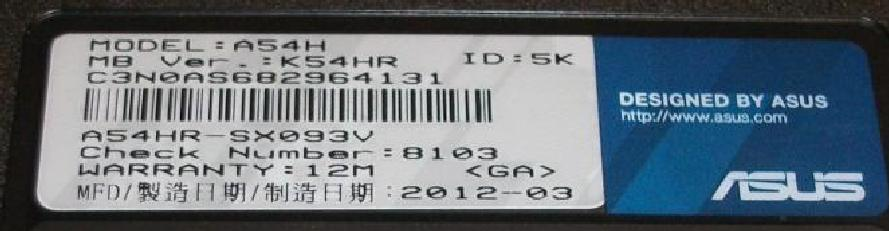
\includegraphics[width=0.4\linewidth]{pics/label1}};
%							\label{fig:label1}
%					\end{tikzpicture}
				\item impacchettare con cura ed etichettare i plichi;
				\item \textbf{cercare password, PIN, appunti;}
				\item valutare la necessità di rilievi dattiloscopici.
			\end{itemize}		
		In questa fase inizia la \textit{catena di custodia} del materiale fisico.
		\begin{figure}
			\centering
			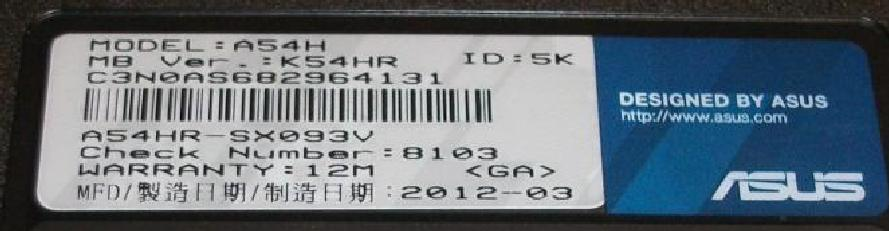
\includegraphics[width=0.6\linewidth]{pics/label1}
			
			\label{fig:label1}
		\end{figure}

			
	\end{frame}
	
	\begin{frame}
		\frametitle{Si può obbligare qualcuno a rivelare una password?}
		
		Nel corso della perquisizione potrà essere chiesto di rivelare password, PIN o altre informazioni utili per accedere ai dati.
		\vfill
		La P.G. è tenuta ad informare sul diritto a non rispondere di cui agli artt. 60 co. 3 e 350 c.p.p., altrimenti il dato ottenuto sarà \textbf{inutilizzabile}.
		\vfill
		\centering
		\Large\textbf{``Nemo tenetur se detegere''}
		
		\scriptsize(nessuno può essere obbligato ad autoaccusarsi)
		
	\end{frame}
	
	\begin{frame}
		\frametitle{Caso 2: computer acceso}

		Come procedere:
		\begin{itemize}
			\item \textbf{non staccare subito la spina:} si perderebbero dati preziosi;
			\item visualizzare ``a mano'' finestre aperte, pagine web attive, processi, ecc. o con apposito software;
			\item documentare tutta l'attività svolta sul computer, anche filmando il monitor e registrando una nota vocale che descriva le operazioni (come nei film americani!). 
			
		\end{itemize}
		\vfill
		\textit{Ogni atto svolto con queste modalità è di natura irripetibile!}

		\vfill
		Terminate le operazioni di \textit{``live forensic''} si può spegnere il dispositivo: \textbf{staccando la spina e MAI effettuando la procedura di arresto prevista dal sistema operativo!}
	\end{frame}
	
	\begin{frame}
		\frametitle{Sincronizziamo gli orologi}
		Qualora si operi su un dispositivo acceso, vanno sempre annotate l'ora e la data correnti del sistema, rapportandole a quelle effettive dell'intervento.
		\begin{figure}
			\centering
			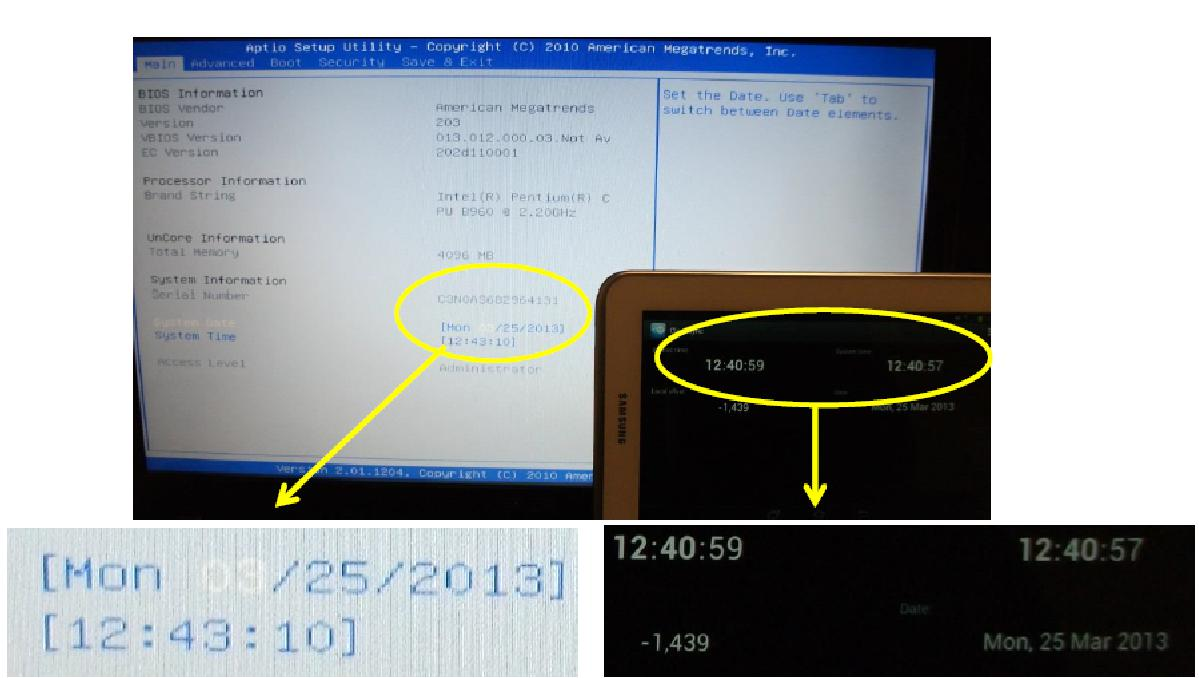
\includegraphics[width=0.6\linewidth]{pics/dataora}
			\label{fig:dataora}
		\end{figure}
		Questo è di fondamentale importanza per mettere in relazione gli orari delle operazioni della P.G. con i dati che verranno estratti dall'analisi \textit{post mortem}.
	\end{frame}
	
	\begin{frame}
		\frametitle{Caso 3: server o apparecchiatura di rete}
		
		Come mettere in sicurezza dati conservati su un server:
		
		\begin{itemize}
			\item capire se l'apparecchiatura in questione sia o meno nella completa disponibilità dell'indagato;
			\item limitare i ``danni collaterali'' provocati a persone non coinvolte nell'attività dell'indagato;
			\item se non è presente un tecnico, affidarsi all'amministratore del sistema per estrapolare al meglio il materiale di interesse.
			
		\end{itemize} 		
		Sequestrare tutto per poi scremare \textit{a posteriori} può andare bene per i computer  di una privata abitazione: fermare l'attività di un'azienda, incolpevole delle attività criminali degli utenti, dimostra una mancanza di professionalità. 
		\vfill
		\textbf{Non dimenticare mai che più materiale viene sequestrato, più dati si devono analizzare!}
		
	\end{frame}
	\section{Dispositivi mobili}
	\begin{frame}
		\frametitle{Come operare sui dispositivi mobili}
		I dispositivi mobili sono sempre più simili a computer che non a semplici dispositivi di comunicazione quali erano i ``vecchi'' cellulari: ormai, infatti, \textit{smartphone} e \textit{tablet} hanno capacità di archiviazione tra i 32 o 64 GB dei modelli di punta e i 4-8 GB dei modelli più economici. Possono contenere moltissime informazioni e il loro uso pervasivo fa si che, molto più del PC di casa, siano la principale piattaforma di archiviazione dati degli utenti.
		\vfill
		Le modalità di sequestro di tali apparati necessitano a loro volta di alcuni accorgimenti particolari e richiedono un minimo di preparazione da parte degli operatori.
	\end{frame}
	
	\section{Conclusioni}	
	\begin{frame}
		\frametitle{Ringraziamento}
		\centering
		\Large Grazie per l'attenzione.
		\vfill
		\dots e ora: \textit{question time}!
		\vfill	
		\tiny \textbf{Nota:} questa presentazione \textbf{non} è stata realizzata con Microsoft~Powerpoint\textsuperscript\textcopyright bensì con \textsf{\LaTeX}.
	\end{frame}
	
	\begin{frame}
		\frametitle{Riferimenti}
		\tiny
		\bibliographystyle{plain}
		\setbeamertemplate{bibliography item}{\insertbiblabel}
		\bibliography{forensics}
	\end{frame}
\end{document}